\documentclass[sigconf,nonacm,screen,pbalance]{acmart}

\usepackage{enumitem}
\usepackage{soul}
\usepackage{xurl}

\begin{document}
\title{Design and Redesign in Data Visualization}
\author{Fernanda Viégas / Martin Wattenberg}
\maketitle

{\em first published in Malofiej 22, Annual Book}

Visualization is now a mass medium. It's not quite Hollywood,
but information graphics have millions of viewers, awards ceremonies, and even their own
celebrities with tens of thousands of Twitter followers. More important, from the
perspective of journalism, is that data visualization is an essential part of the
communication process. Today, a data-driven story without a chart is like a fashion story
without a photo.

Along with the glitter and popularity, visualization has
attracted something else: popular criticism. It's happening at a small scale; we don't yet
see infographics reviews in the {\em New York Times} Arts section.
Nonetheless, when a striking visualization comes out, it's not unusual to see commentary
and controversy on the web, moving from blogs to Twitter to Facebook. That level of
critique comes with the territory for any popular medium of communication, and shouldn't
be a surprise.

But the process of giving and even receiving visualization
criticism does turn out to hold surprises. It's not just that visualization is so new, or
that criticism can stir up emotions in any medium. As we'll discuss, the fact that
visualizations are based on transforming raw data means that criticism can take forms that
would be impossible for a movie or book. Our goal in this essay is to think through the
issues involved in public visualization criticism, especially criticism based on direct
redesigns.

\section{Redesign as criticism}
We'll begin with a famous critique from a famous critic.
Edward Tufte, in his landmark book Visual Explanations [1], wrote about the decision
process that led to the explosion of the Space Shuttle {\em Challenger} in
1986. Engineers and government officials alike used crude hand-written tables and diagrams
to reason about the situation and communicate their decisions. Tufte provides a masterly
analysis of problems both in the diagrams and the mental process they reflected.

An essential part of Tufte's argument is that design
mattered: the data was sufficiently conclusive that with clear communication based on
clear thinking, the shuttle would never have launched. (Depressingly, he makes the case
that even the report produced after the failure embodied muddled thinking.) To prove his
point about design, Tufte produced a redesign, a new diagram that's a paragon of clarity
compared to the original tables produced by engineers or the charts seen in the official
government investigation.




\begin{figure*}[ht]
\centering
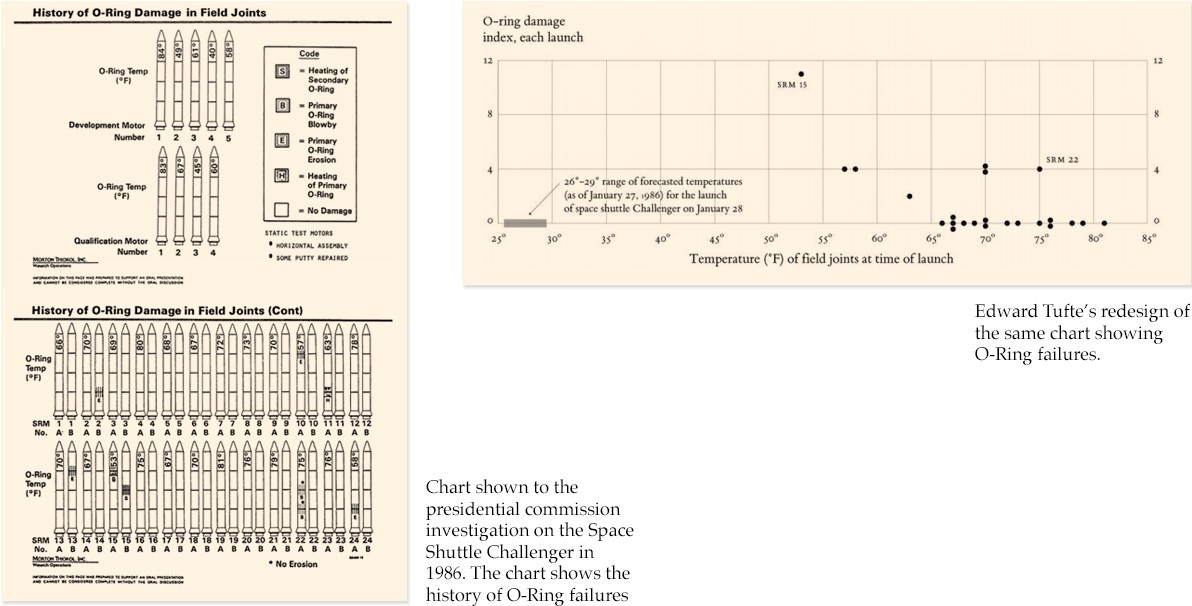
\includegraphics[width=\textwidth]{1_iQcNh732KTyKd6qROcebhg.jpg}
\end{figure*}


To demonstrate how the key variables could be directly
compared, Tufte produced the scatterplot in the figure above. In this chart, the data
seems to speak for itself: an unmistakable illustration of the danger of low temperatures,
with the only cold-weather launch appearing as a clear outlier. The scatterplot redesign
is one part of long and subtle analysis, but it has pride of place. ``Had the correct
scatterplot or data table been constructed,'' concludes Tufte, ``no one would have dared to
risk the Challenger in such cold weather.''

The tradition of critique by redesign is, if anything,
growing in popularity. Here's very recent example. Giorgia Lupi, of Accurat, created a
diagram of the output of famous authors, visualizing the dates of their masterpieces in
the context of their lifespans. Her chart was an unusual combination of ``small multiple''
polygons that encoded several different publications for each author. Alberto Cairo, a
professor at University of Miami, used straightforward linear timelines based on the same
data. The resulting side-by-side comparison [2] makes it extremely easy to compare the two
encoding methods.


\begin{figure*}[ht]
\centering
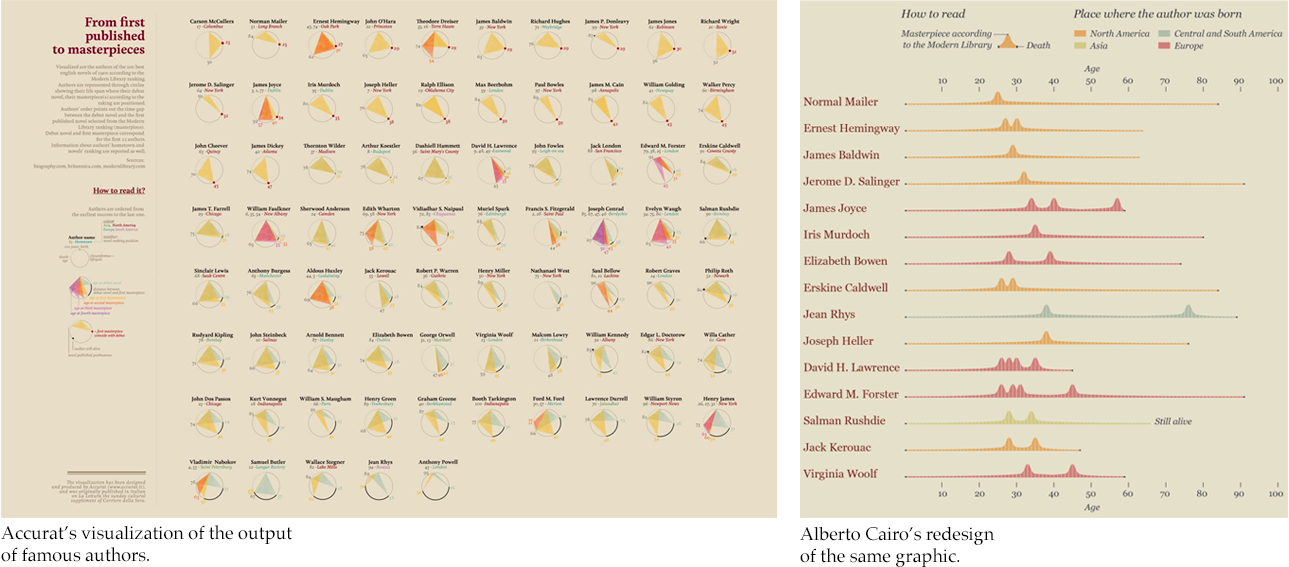
\includegraphics[width=\textwidth]{1_1w9irsLhPVwMdUrLPJXs-A.png}
\end{figure*}


\hl{The technique of ``critique by
redesign'' in some ways works uniquely well in data visualization.} A movie critic
can't remake a movie. An art critic can't ask the subject of a portrait to sit for a
second time. A book critic may be able to rewrite a sentence, but not a whole book. But
with data visualization, if there's access to the underlying data set, and the data is not
too complicated, it's feasible to create at least a rough redesign.

Of course, just because this technique is feasible doesn't
mean it's a good thing. The implications of critique by redesign are surprisingly complex,
and we'll spend much of this essay unpacking them. But even these initial examples show
some of the obvious advantages and drawbacks.

First, some advantages. A redesign is -- or should be --
intellectually honest, since it's using the same data. It also allows direct visual
comparison; when a visualization is described in words, something is always lost in
translation. Enabling direct, honest comparisons leads to the second key advantage, which
is that redesigns are convincing in a democratic way. Instead of a verbal appeal to
authority (``This design is flawed because I say so'') a side-by-side comparison lets the
viewer decide.

At the same time, redesigns can be problematic. Tufte had one
huge advantage over the creators of the diagrams used to make the space shuttle decision:
he knew the answer to the question they were considering, and he knew exactly which
variables mattered. His redesign makes an open-and-shut case at first glance. Stare a
little longer, and you realize that the bulk of the visual effect rests on just one data
point, the dramatic outlier at the upper left corner. Remove that, and the trend takes a
far more muted form. Would it have convinced a stubborn politician to call off the launch?


Indeed, is it really a good idea to give so much weight to a
single outlying data point? Clearly in the case of the {\em Challenger} it
would have been. As a general rule, though: not always. One wonders... Had the launch gone
off without incident, could someone with Tufte's skill have created, from the same data,
an equally convincing graphic about the wisdom of ignoring outliers?

Tufte also took a second shortcut. His scatterplot picked out
the exact data dimensions that -- after the fact -- were known to be decisive. It leaves out
variables such as the location or type of O-ring problems. In hindsight, that information
was irrelevant to the analysis, but of course there was no way to know that at the time.
Adding that data to the chart would have made it more cluttered and ambiguous. In fact,
it's all too common to see critics simplify in ways that help their cases. Cairo's
redesign of Lupi's timeline is airy and elegant... but only shows 50\% of the data in the
same space. In these particular cases, the shortcuts don't seriously undermine the
critics' main points, but they do raise some room for doubt.

Perhaps the biggest problem with redesigns, however, is their
removal of context. Design is compromise. Anyone who's ever designed a logo, made a movie,
or built a house, knows that the final product reflects a series of mostly hidden goals
and constraints. To redesign without knowing these constraints -- the client insisted on
pink! the lead actor broke his ankle! the zoning board was insane! -- is, in some sense,
unfair.

In the case of visualizations, this context can range from
differences in strategy and goals to tactical constraints. As Tufte discusses,
{\em Challenger}'s engineers were well aware of the risks of the flight and
had recommended against launching. However, political pressure around the timing may have
made the difference in the decision. Despite his conclusion that the right scatterplot or
data table would have made the difference, the best design in the world might not have
changed the decision. In the case of Cairo's redesign, the relative weight placed on
legibility versus aesthetics and novelty may have been different.

It should be clear by now that there's no such thing as a
simple redesign.

\section{Redesign in public}
In 2004 the U.S. electorate was dramatically divided between
two presidential candidates: President George Bush from the Republican Party and John
Kerry from the Democratic Party. Throughout the campaign, election maps tracked the split,
with ``red'' and ``blue'' states representing locations whose residents predominantly voted
for the Republican Party (red) or Democratic Party (blue). A major flaw of the red-blue
map was the impression it gave that the Republican Party had a much wider following than
it actually did. Because of the large geographical size of many states in the central and
southern United States, which predominantly supported the Republican candidate, the
color-coded map ended up as a sea of red. The impression was of a country that
overwhelmingly voted Republican. In other words, the map
failed to take into account the population distribution of the U.S. It did not capture the
fact that population in red states is, on average, significantly lower and less dense than
that of blue states (more Democrat voters tend to live in large cities).

\begin{figure}[ht]
\centering
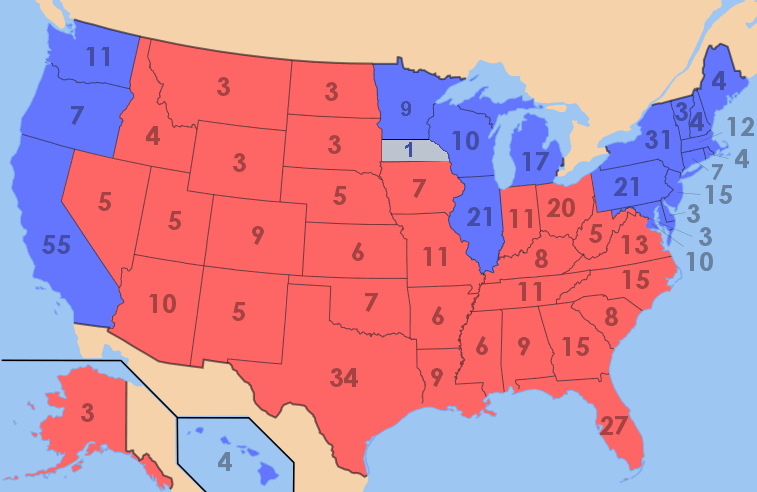
\includegraphics[width=\columnwidth]{1_7rY2a4CFDnJO2GmtoS37qQ.png}
\vspace{-20pt}
\caption{Red and Blue Map of 2004 US Presidential Election. (Election maps from Wikipedia [4])}
\end{figure}
This visual puzzle generated a public quest for more
effective ways of displaying U.S. election data. Data scientists, journalists, and
visualization experts among others produced a series of maps that tackled different angles
of the problem. County-based maps broke down states into smaller units so that pockets of
Democratic voters could be seen in Republican states. ``Purple haze'' maps blended red and
blue reflecting the percentage of Republican and Democratic votes in each location.
Cartograms, a more exotic technique from the world of data visualization, distorted
geographical areas by scaling counties and states according to their population.

\begin{figure*}[ht]
\centering
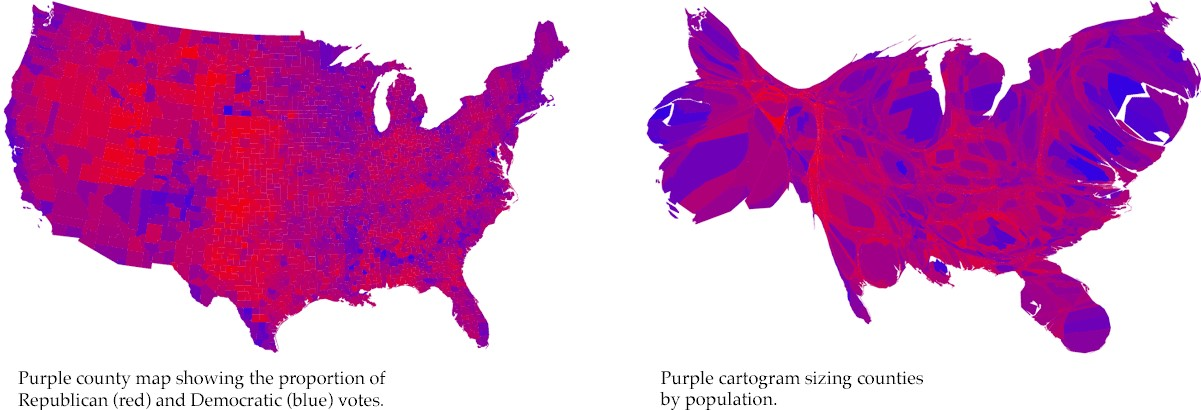
\includegraphics[width=\textwidth]{1_HRfH95w8UVsKETopIN14lQ.jpg}
\end{figure*}


This process of data analysis and map creation happened in
public, with different versions of the ``Red and Blue'' map appearing every few weeks. There
was no single right answer to speak of. Each map represented a series of tradeoffs and
biases. In aggregate, though, these maps constituted a dialog; a powerful and healthy new
way of engaging in a public exchange of ideas about a country's identity and direction.
Perhaps just as important, these activities evolved in a fairly collaborative manner.
Instead of trying to explicitly redesign each other's maps, practitioners were building on
each other's work to get to a better visual encoding of the data. It was a collaborative
activity fueled by the need to visualize and understand the data better.

Unfortunately, public re-creations of data visualization
projects may not always lead to such a uniformly positive reaction. There have been
occasions where redesigns met with significant backlash. Take, for example, a second
redesign done by Alberto Cairo in February 2015. As with his critique of Giorgia Lupi's
work, Cairo took a radial plot (a timeline of the Arab Spring timeline, created by
Alexander Katin and Kir Khachaturov) and ``unrolled'' it to linear coordinates.

After Cairo blogged his redesign, responses came fast and
furious, falling mostly along two opposing lines, one arguing for the importance of
aesthetics in the original graph, the other contending that data legibility was
dramatically improved in the redesigned solution.




\begin{figure*}[ht]
\centering
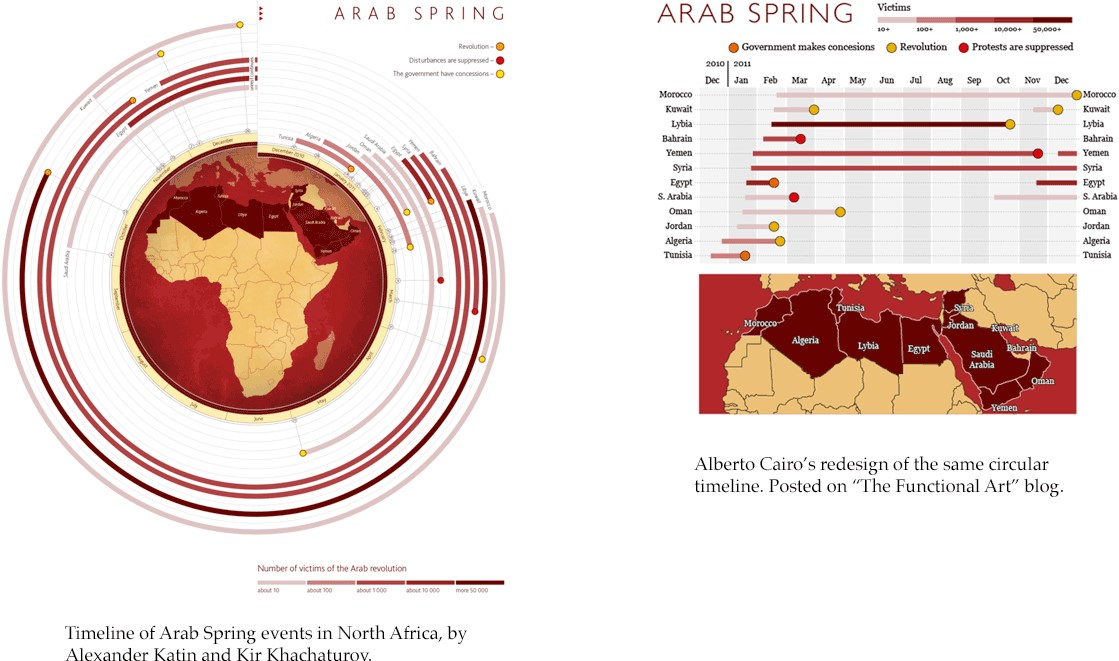
\includegraphics[width=\textwidth]{1_xIjO8n-Pp0Z4q1puoavP2g.jpg}
\end{figure*}


\begin{quotation}
    {\em ``@albertocairo The circle is meant to show a
    yearly cycle, right?''}
    
    {\em ``The distortion caused by the circular
    layout makes the timeline of Tunisia looks shorter than that of Yemen, when in fact
    the period depicted for Yemen is much shorter''}
    
    {\em ``I'm siding with @blprnt rather than
    @albertocairo in the great circular timeline debate of 2015.''}
    
    {\em ``I'm with the straight line version, if the
    purpose is clarity. To read the circles I need to perform, like, a zillion eye
    movements as a I move along the scale.''}
    
    Sample quotes from Twitter. In addition to the passages
    above, there were some more heated Tweets as well (all caps and expletives).
\end{quotation}

Public redesigns that are broadcast to thousands, potentially
millions of people around the world are a new phenomenon, a product of the social media
era. Such reach and immediacy can have both benefits and disadvantages. On the plus side,
it is easy and cheap for redesigns to be widely seen and discussed by the data
visualization community. On the other hand, because they take place on social media, such
redesigns automatically collapse multiple audiences into a single context. It is a stark
departure from traditional design-studio-based peer crits where colleagues share the
context and intent of a piece, know the person whose design is being critiqued, and are
physically present. Online, public redesigns can feel faceless and less personal, quickly
inviting animosity and bitterness.

In the Cairo example, the initial context was pedagogical:
his student had asked about radial graphs and Cairo was hoping to illustrate the
effectiveness of linear versus radial solutions. Once on Twitter though, the conversation
took on a different tone, including questions about aesthetics, Cairo's authority in the
subject matter, the importance (or lack thereof) of the data shown, the role of design,
etc. On the one hand, this broadening of topics is something to aspire to during a
critique. On the other, the antagonism that sometimes accompanies such exchanges would be
better left out of the process altogether. But how to balance these tradeoffs: reach vs.
context? And how to optimize so that most of the discussion around a redesign is
productive?

\section{Redesign: bridging the two
cultures}
The field of visualization sits at the intersection of two
very different intellectual traditions. On one side of the family, visualization traces
its roots to art and graphic design. On the other side, it's descended from computer
graphics and the tradition of scientific experiment. It's worth taking a step back and
describing some of the morés and norms in each field, and how they conflict in the case of
visualization criticism.

An essential way that literary and artistic fields move
forward intellectually is {\em criticism}. Colloquially, ``criticism'' implies
negativity, but of course there's a much richer tradition in the arts and humanities. As
Bardzell puts it, ``{\em Speaking generally, criticism refers to an expert of a
given domain's informed exercise of judgment; familiar examples include film and
literary critics, architectural criticism, and even a qualified Master of Wine's ability
to judge wine.}'' [3] One reason to emphasize this definition is to avoid a trivial
misunderstanding: an endorsement of ``visualization criticism'' isn't a call for general
negativity.

In the design community, there's a particular flavor of
criticism that is common: the design critique. Unlike more abstract or philosophical
literary criticism, a classic ``crit'' usually has the goal of improving a work in progress.
A key part of the critique process is the social context: the fact that it's a group of
colleagues having a serious, high-level conversation. It's rare for a crit to be held in
public; they're more commonly found in studios and schools, comprised of professionals and
students -- people dedicated to their craft, with a shared knowledge of the context for a
design, exercising careful judgment.

In science, we see something different. Science seeks to
remove human judgment from the process of testing hypotheses. (Judgment certainly survives
in funding and publication processes, but that's a separate story.) A hypothesis isn't
even considered scientific unless it's falsifiable, that is, there's a mechanical recipe
for showing it's wrong. The gold standard for a new medical treatment, after all, isn't
the opinion of a committee of doctors, but a double-blind experiment -- ideally, an
experiment that is replicated successfully by more than one group.

In the case of computer graphics, one of the scientific
ancestors to data visualization, we see a series of test images that have become de facto
standards. For instance, researchers who work on 3D rendering often start with a
particular teapot model. Scholars of image compression and enhancement have for decades
used the (notorious) ``Lena'' {\em Playboy} portrait. The goal is to apply new
techniques and ideas in a well-understood context, so anyone may perform a direct
comparison with previous work.

Comparing these traditions explains some sources of confusion
in criticism by redesign. Seen from a tradition where critique largely happens in private,
a public redesign can feel unduly personal and exposed. A critique that happens in public,
available to anyone who clicks the right link, loses much of the context necessary for
thoughtful commentary. Meanwhile, from the point of view of an experimental scientist, the
necessary human -- and ultimately subjective -- professional judgment that is involved in
evaluating a redesign may seem like a cheat. We've seen evidence of both these reactions
from practitioners in the field.

Despite these issues, the method of ``critique by redesign''
may be just the blend that will help advance the field. The truth is that perceptual
psychology and related sciences can provide some guidance for visualization, but are
nowhere near advanced enough to completely answer all real-world design questions.
Ultimately, human judgment remains essential to the process. And while the lack of context
and collegiality can make a public critique problematic, we believe there are ``rules of
engagement'' that can bring out the best in the process and avoid some of the worst
pitfalls.

\section{Rules of engagement}
Design is not a science. But ``not a science'' isn't the same
as ``completely subjective''. In fact, the critique process has brought discipline to design
for centuries. For visualizations which are based on an underlying shared data set,
there's an opportunity for an additional level of rigor: to demonstrate the value of a
critique through a redesign based on the same data.

Criticism through redesign may be one of the most powerful
tools we have for moving the field of visualization forward. At the same time, it's not
easy, and there are many pitfalls, intellectual, practical, and social. How can we use the
tool of criticism to best advantage, with awareness and respect for all involved? Here are
some suggestions, which fall into three categories: maintain rigor, respect for designers,
and respect for critics.

\subsection{Maintain rigor}
As with a scientific experiment, it's important to know the
reason for a redesign -- what is being ``measured'', in a sense. There are many possible
goals for a visualization: to communicate data, to spur conversation, to persuade, to draw
in viewers, to create an aesthetic experience. A critic who creates a redesign should be
explicit about the goal -- and the fact that they may be interested in a different goal
than the designer. This is especially important on the web, where people may stumble on
the result without knowing any other context.

Second, critics must be honest about any simplifying
assumptions. If a redesign shows less data than the original, that should be mentioned up
front. Otherwise, there's a danger that any perceived simplicity of a redesign is really
just the result of a reduction in data.

Part of maintaining rigor is acknowledging situations where
professional judgments don't agree, and finding ways to come to an understanding.
Sometimes people will look at a side-by-side comparison and come to opposite conclusions.
(We saw this in the radial timeline redesigned by Alberto Cairo, for example.) The first
step is to have a conversation about the source of the disagreement. Very often it turns
out that different professionals have different criteria for success for a visualization,
or have different goals in mind; clarifying these is extremely useful to the field. Other
times, however, people simply have different intuitions about clarity or legibility. In
these situations, it may make sense to turn to a scientific experiment. This should not be
viewed as a failure of criticism, but rather a success: a crisp, testable scientific
question is a rare commodity.

\subsection{Respect the designer}
All redesigns have the potential to seem adversarial, as if
the critic is pointing out flaws in the designer personally, asserting their own superior
skills, or even, as in Tufte's redesign, assigning some blame for a disaster. In the age
of viral links, the effect is doubled: seeing negative comments about your own work being
reblogged, retweeted, and reposted isn't a pleasant experience.

Making the process more friendly for the designer is good for
many reasons. It's kind, of course. Beyond that, it opens up the possibility of a
conversation. Often the original designer of a piece has thought more about its particular
problems than anyone else. We recommend bringing the designer into the conversation at
every level: talking with them in advance about a public critique, giving them a chance to
respond, and at every turn treating them as a competent professional.

Critics can take many steps to soften the emotional impact of
redesigns on the designer.

First, if you could make a point by criticizing several
different visualizations, pick whichever comes from an organization with the highest
prestige. If you have to point out flaws publicly, it's better to do it to the {\em New York Times} than a first-year student. It's not always true that more
established designers have thicker skin, but they ought to. Second, if it makes sense in
the context of a critique, note the positive aspects of a design -- that is, the features
that need no redesign. If the color and typography are excellent and need no change, it
might be a good idea to call that out.

Third, to make pedagogical points, consider a ``backwards''
redesign, one that takes an excellent visualization and makes it worse. In other words,
take a visualization that exemplifies the point you're trying to make (say, good labeling
or a good color palette) and then remove key elements (most of the labels, or change
colors to vibrate against one another). This may give you the same effect as a traditional
redesign, but leave the original designer flattered rather than aggrieved. It's also a
good way to move past the idea that ``criticism'' implies a negative view of existing work.


\subsection{Respect the critic}
Criticism is hard, as hard as design. Indeed, in established
media (books, movies, music) good critics are recognized as experts in their own right. As
a field, we should give the same respect to our visualization critics. One occasionally
hears designers complain that a critic isn't an active practitioner. Well, that may be
true, but it shouldn't matter.

As a consequence, we shouldn't let some roughness in a
redesign be an excuse to ignore it. A redesign doesn't need to be perfectly polished to be
effective. It may even be better for it to be slightly rough. After all, a redesign isn't
a competition between critic and designer, but instead a proof point for ideas about
design.

A final point for designers is to keep in mind the goal of
the critique process: ultimately, none of this is a personal evaluation, but instead a way
for the field as a whole to improve.

\section{Conclusion}
Data visualization is still a new field. It's already become
an essential medium for journalists, scientists, and anyone else who needs to understand
data. But the medium is far from understood. It's early still, and there's a lot of room
for improvement.

We need more criticism, and redesign is an essential part of
visualization criticism. But with so much of it happening on the web -- in public,
instantly in view of everyone involved, available to the world without context or
preparation -- it can be a difficult process. In this chapter our goal has been to start a
conversation about how criticism can be most productive, and cause the least stress, for
those involved.

We'd like to end with a thought about the future. The
redesigns and criticism we've discussed have very much been focused on technique. That's
appropriate for a new medium in its growth phase. Compared to criticism of movies or
books, however, it's unusual. Think of a typical book review: certainly writing style and
form figure in reviews. But usually at least as much space, often much more, is given to
questions of content: to character, to plot, to atmosphere. We'll know that visualization
has matured as a medium when we see as much criticism about content as we do today about
technique.

\begin{acks}
Following our own precepts, we've tried to make this essay
part of a larger conversation. The impetus came from an online critique by Alberto Cairo,
along with discussion that followed on Twitter, blogs, and email. In particular we'd like
to thank Moritz Stefaner, Jan Willen Tulp, and others for helpful discussions and
pointers.
\end{acks}

\bibliographystyle{ACM-Reference-Format}
\bibliography{references}

[1] Visual Explanations: Images and Quantities, Evidence and Narrative.

[2] \url{http://www.thefunctionalart.com/2014/11/redesigning-visualizations.html}

[3] J. Bardzell / Interacting with Computers 23 (2011) 604–621

[4] \url{http://en.wikipedia.org/wiki/File:2004_US_elections_map_electoral_votes.png}

\url{http://commons.wikimedia.org/wiki/File:Gastner_map_purple_byarea_bycounty.png}

\url{http://commons.wikimedia.org/wiki/File:Countycartlinear1280x1024.png}
\end{document}
\endinput